%%
%  ******************************************************************************
%  * #file    Szablon_raportu_EN_Latex.tex
%  * #author  Adrian Wójcik   adrian.wojcik(at)put.poznan.pl
%  *          
%  * #commit  Patryk Kościk   koscikpatryk(at)gmail.com
%  *          Modified the template for Projekt przejsciowy purposes          
%  *          
%  * #version 1.0
%  * #date    09-Mar-2022
%  * #brief   PROJPRZEJ
%  *
%  ******************************************************************************
%%  
\documentclass[11pt, a4paper]{article}

\usepackage{SM_template}

% Wypełnijcie te dyrektywy zgodnie z waszym tematem
% \lab      -> NAZWA CZUJNIKA, np.: 'DHT22'
% \comment  -> Króciutki opis co to, np.: 'Cyfrowy budżetowy czujnik temperatury'
%
\lab{KY-032}
\comment{Podczerwony czujnik uniku \\ Szymon Kwiatkowski}

% Absolutny zakaz dotykania tego tutaj bo jak dotkiecie to coś jebnie
\university{Politechnika Poznańska}
\faculty{Wydział Automatyki, Robotyki i Elektrotechniki}
\institute{Instytut Robotyki i Inteligencji Maszynowej}
\department{Zakład Sterowania i Elektroniki Przemysłowej}
\addbibresource{bib/KY-032.bib}
\nocite{*}


%%
%
% Początek dokumentu
%
%%
\begin{document}

%% Strona tytułowa %%
\mainpage{{KY-032/KY-032.jpg}}
\newpage

\section*{Opis elementu} \addcontentsline{toc}{section}{Wstęp}
Czujnik jak sama nazwa mówi służy do wykrywania kolizji z potencjalnymi obiektami. Najważniejszymi z parametrów czujnika jakie musimy znać to:
\begin{itemize}
\item Posiada on napięcie zasilania od 3,3V do 5V
\item Jest w stanie dokonać detekcji obiektu w odległości od 20 cm do 40 cm
\item Posiada on 4 piny z czego jeden jest pinem wyjściowym i służy do detekcji obiektu(stan niski obiekt wykryty oraz stan wysoki brak obiketu)
\item Odległość w której wykrywamy obiekt może być dostosowana przez użytkownika za pomocą potencjometru.
\end{itemize}

Moduł wykorzystuje diodę emitującą podczerwień jako czujnik do wykrywania obiektu, który zarówno wysyła jak i odbiera wiązkę pozwalającą na detekcję.  Czujnik posiada domyślnie 4 piny którymi są:
\begin{itemize}
\item GND
\item +(VCC)
\item EN
\item S - sygnał wyjśiowy
\end{itemize}
\begin{figure}[H]
    \centering
    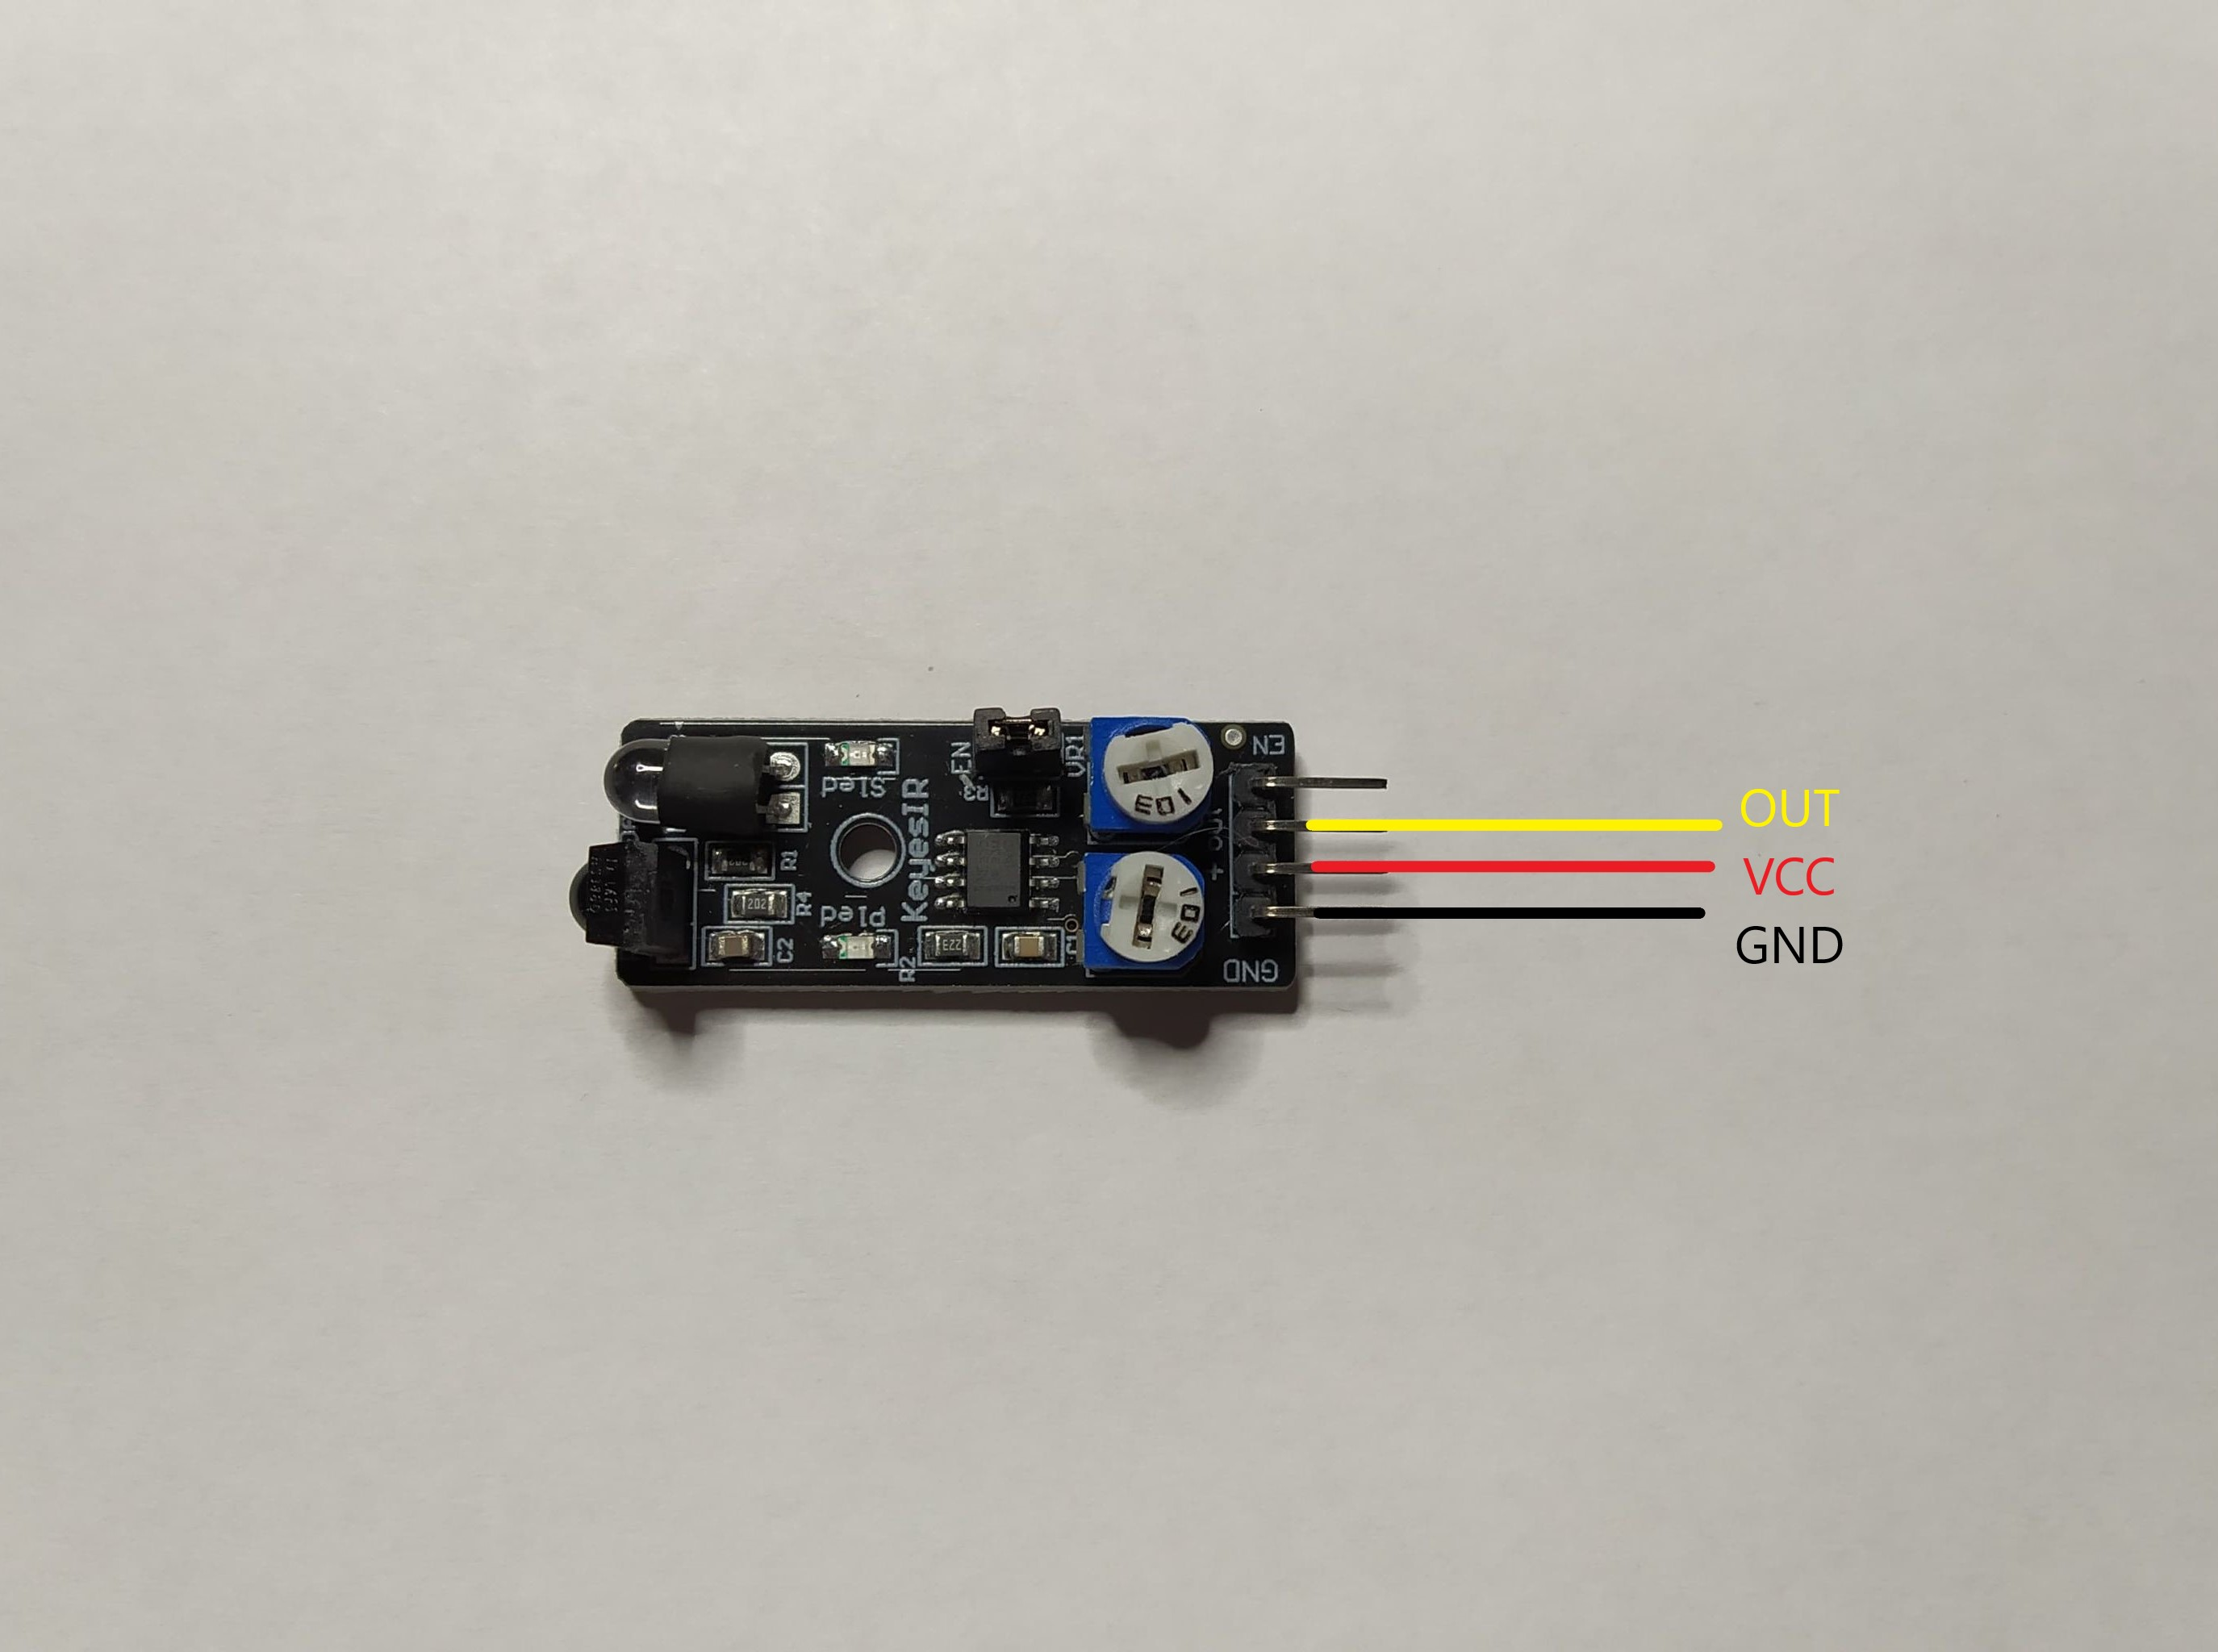
\includegraphics[width=0.7\textwidth]{fig/KY-032/polaczenie_modulu/KY-032_Pins.jpg}
    \caption{Piny wychodzące z modułu}
\end{figure}


Sygnał EN służy do uruchomienia funkcjonalności czujnika związanej z wykrywaniem obiektów jednak domyślnie posiadamy również zieloną zworkę która służy do załączenia tej funkcjonalności na stałe niezależnie od sygnału podanego na EN.
\newline
Dodatkowo jako osoba użytkująca posiadamy opcję dostosowania odległości w której wykrywamy obiekt za pomocą lewego potencjometru który dostraja właśnie odległość(w środkowym położeniu posiadamy największą wartość odległości czyli 40cm). Jest również możliwość dostosowania częstotliwości z jaką wysyłana i odbierana jest wiązka z diody podczerwonej. Można tego dokonać za pomocą prawego potencjometru, który kręcąc zgodnie z ruchem wskazówek zegara może zostać dostrojony do pożądanej wartości częstotliwości.. 
\newline
Schemat samego układu czujnika wygląda następująco:
\begin{figure}[H]
    \centering
    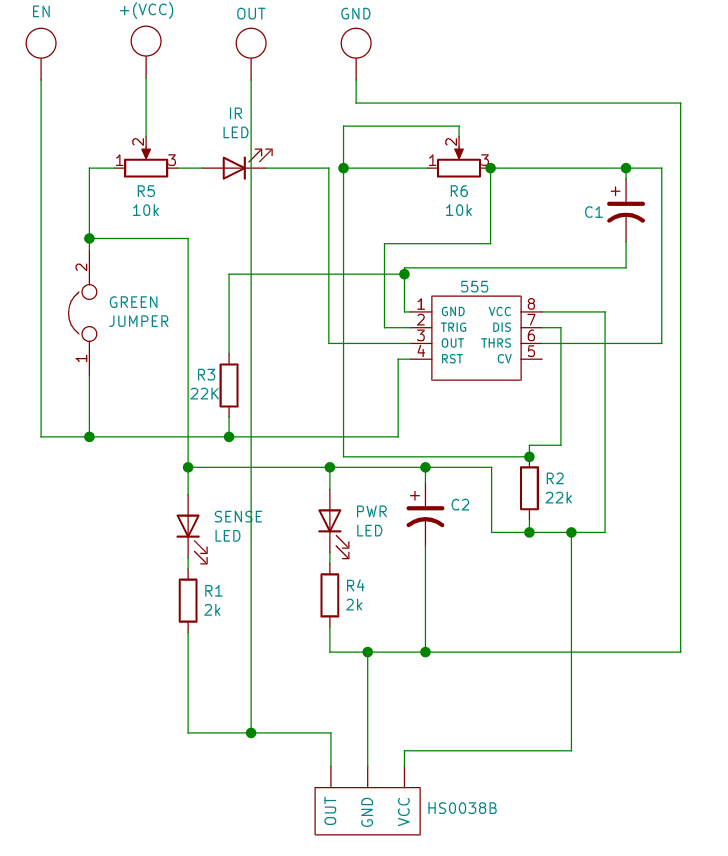
\includegraphics[width=0.7\textwidth]{fig/KY-032/zasada_dzialania/schemat.png}
    \caption{Schemat układu KY-032}
\end{figure}

\newpage

\section{Użycie czujnika}
Czujnik można głównie wykorzystać jako właśnie czujnik wykrycia obiektu. Wykorzystanie detekcji może odbyć się za pomocą prostego sprawdzania stanu pinu GPIO pod który posiadamy wpięte wyjście czujnika S. Jeżeli stan wejścia GPIO jest niski to wiemy że przed nami w zakresie zasięgu ustawionego wewnątrz czujnika znajduje się obiekt. Jeżeli stan ten jest z kolei wysoki to przed nami nie znajduje się żaden obiekt i tym samym możemy łatwo zidentyfikować sytuacje.

Przykładem mogą być poniższe pomiary:
\begin{figure}[H]
    \centering
    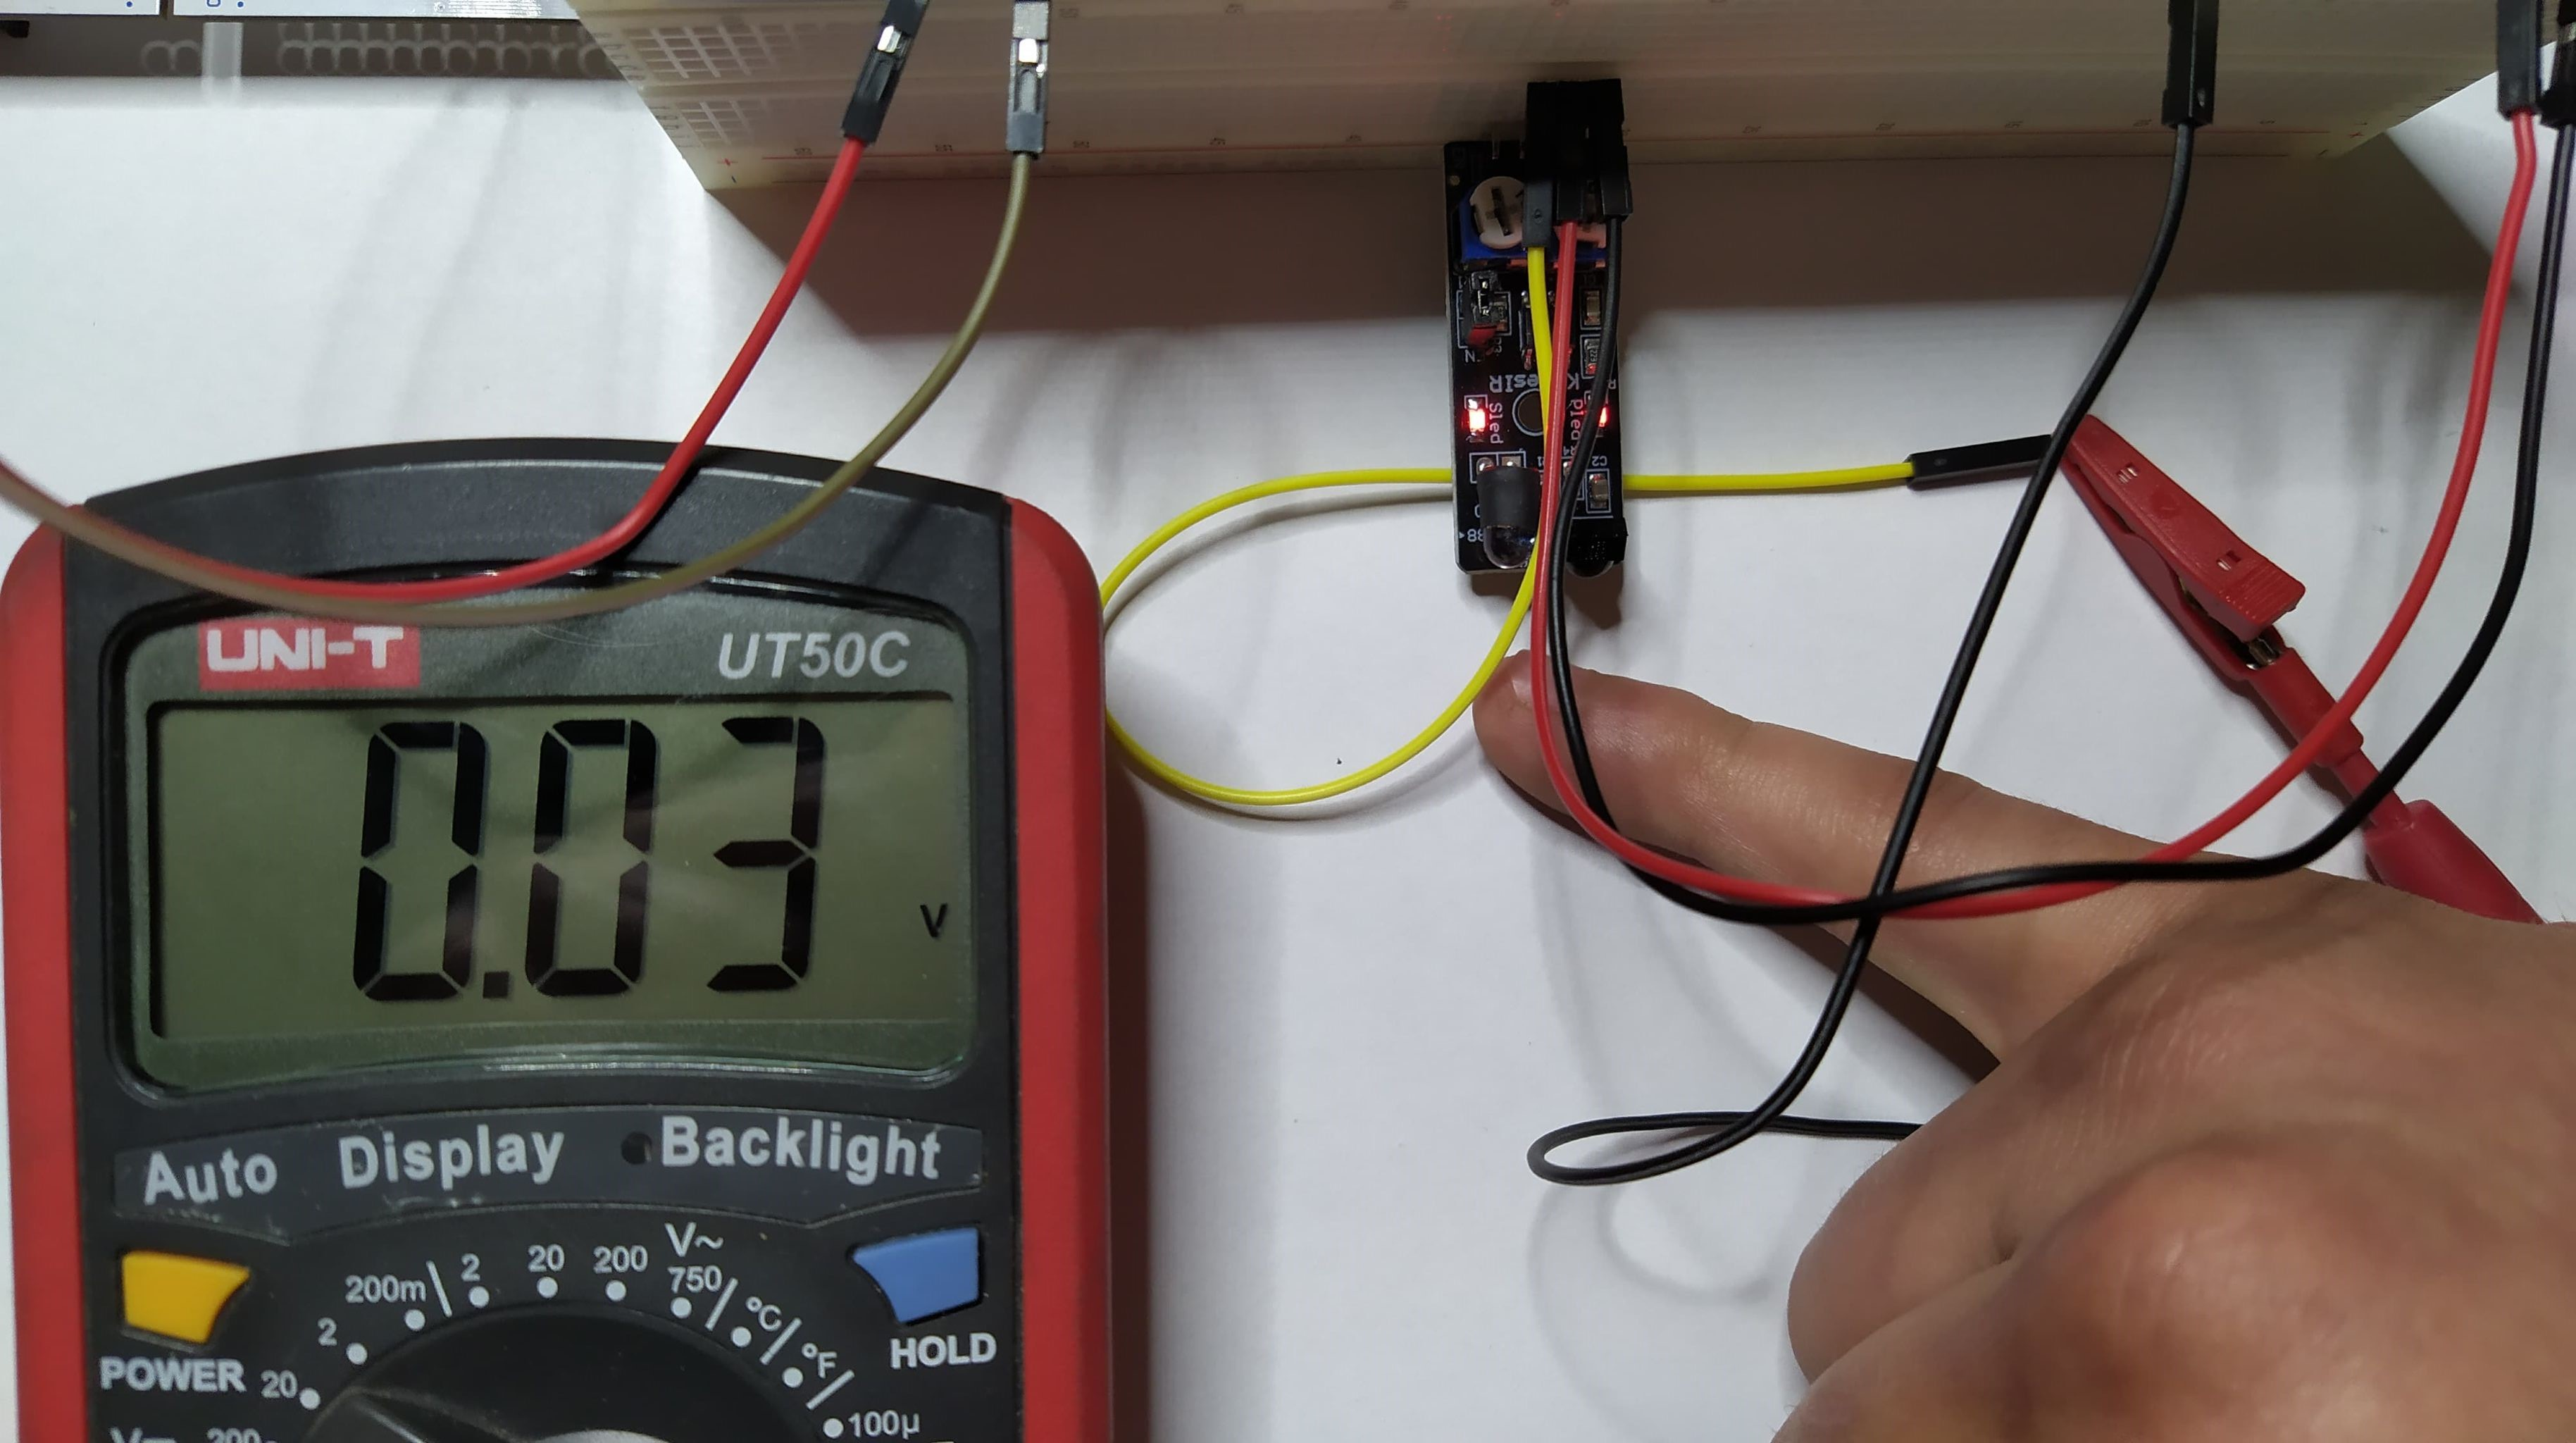
\includegraphics[width=0.7\textwidth]{fig/KY-032/zasada_dzialania/Avoidance_pomiar2.jpg}
    \caption{Pomiar dla obiektu będącego przed czujnikiem}
\end{figure}
\begin{figure}[H]
    \centering
    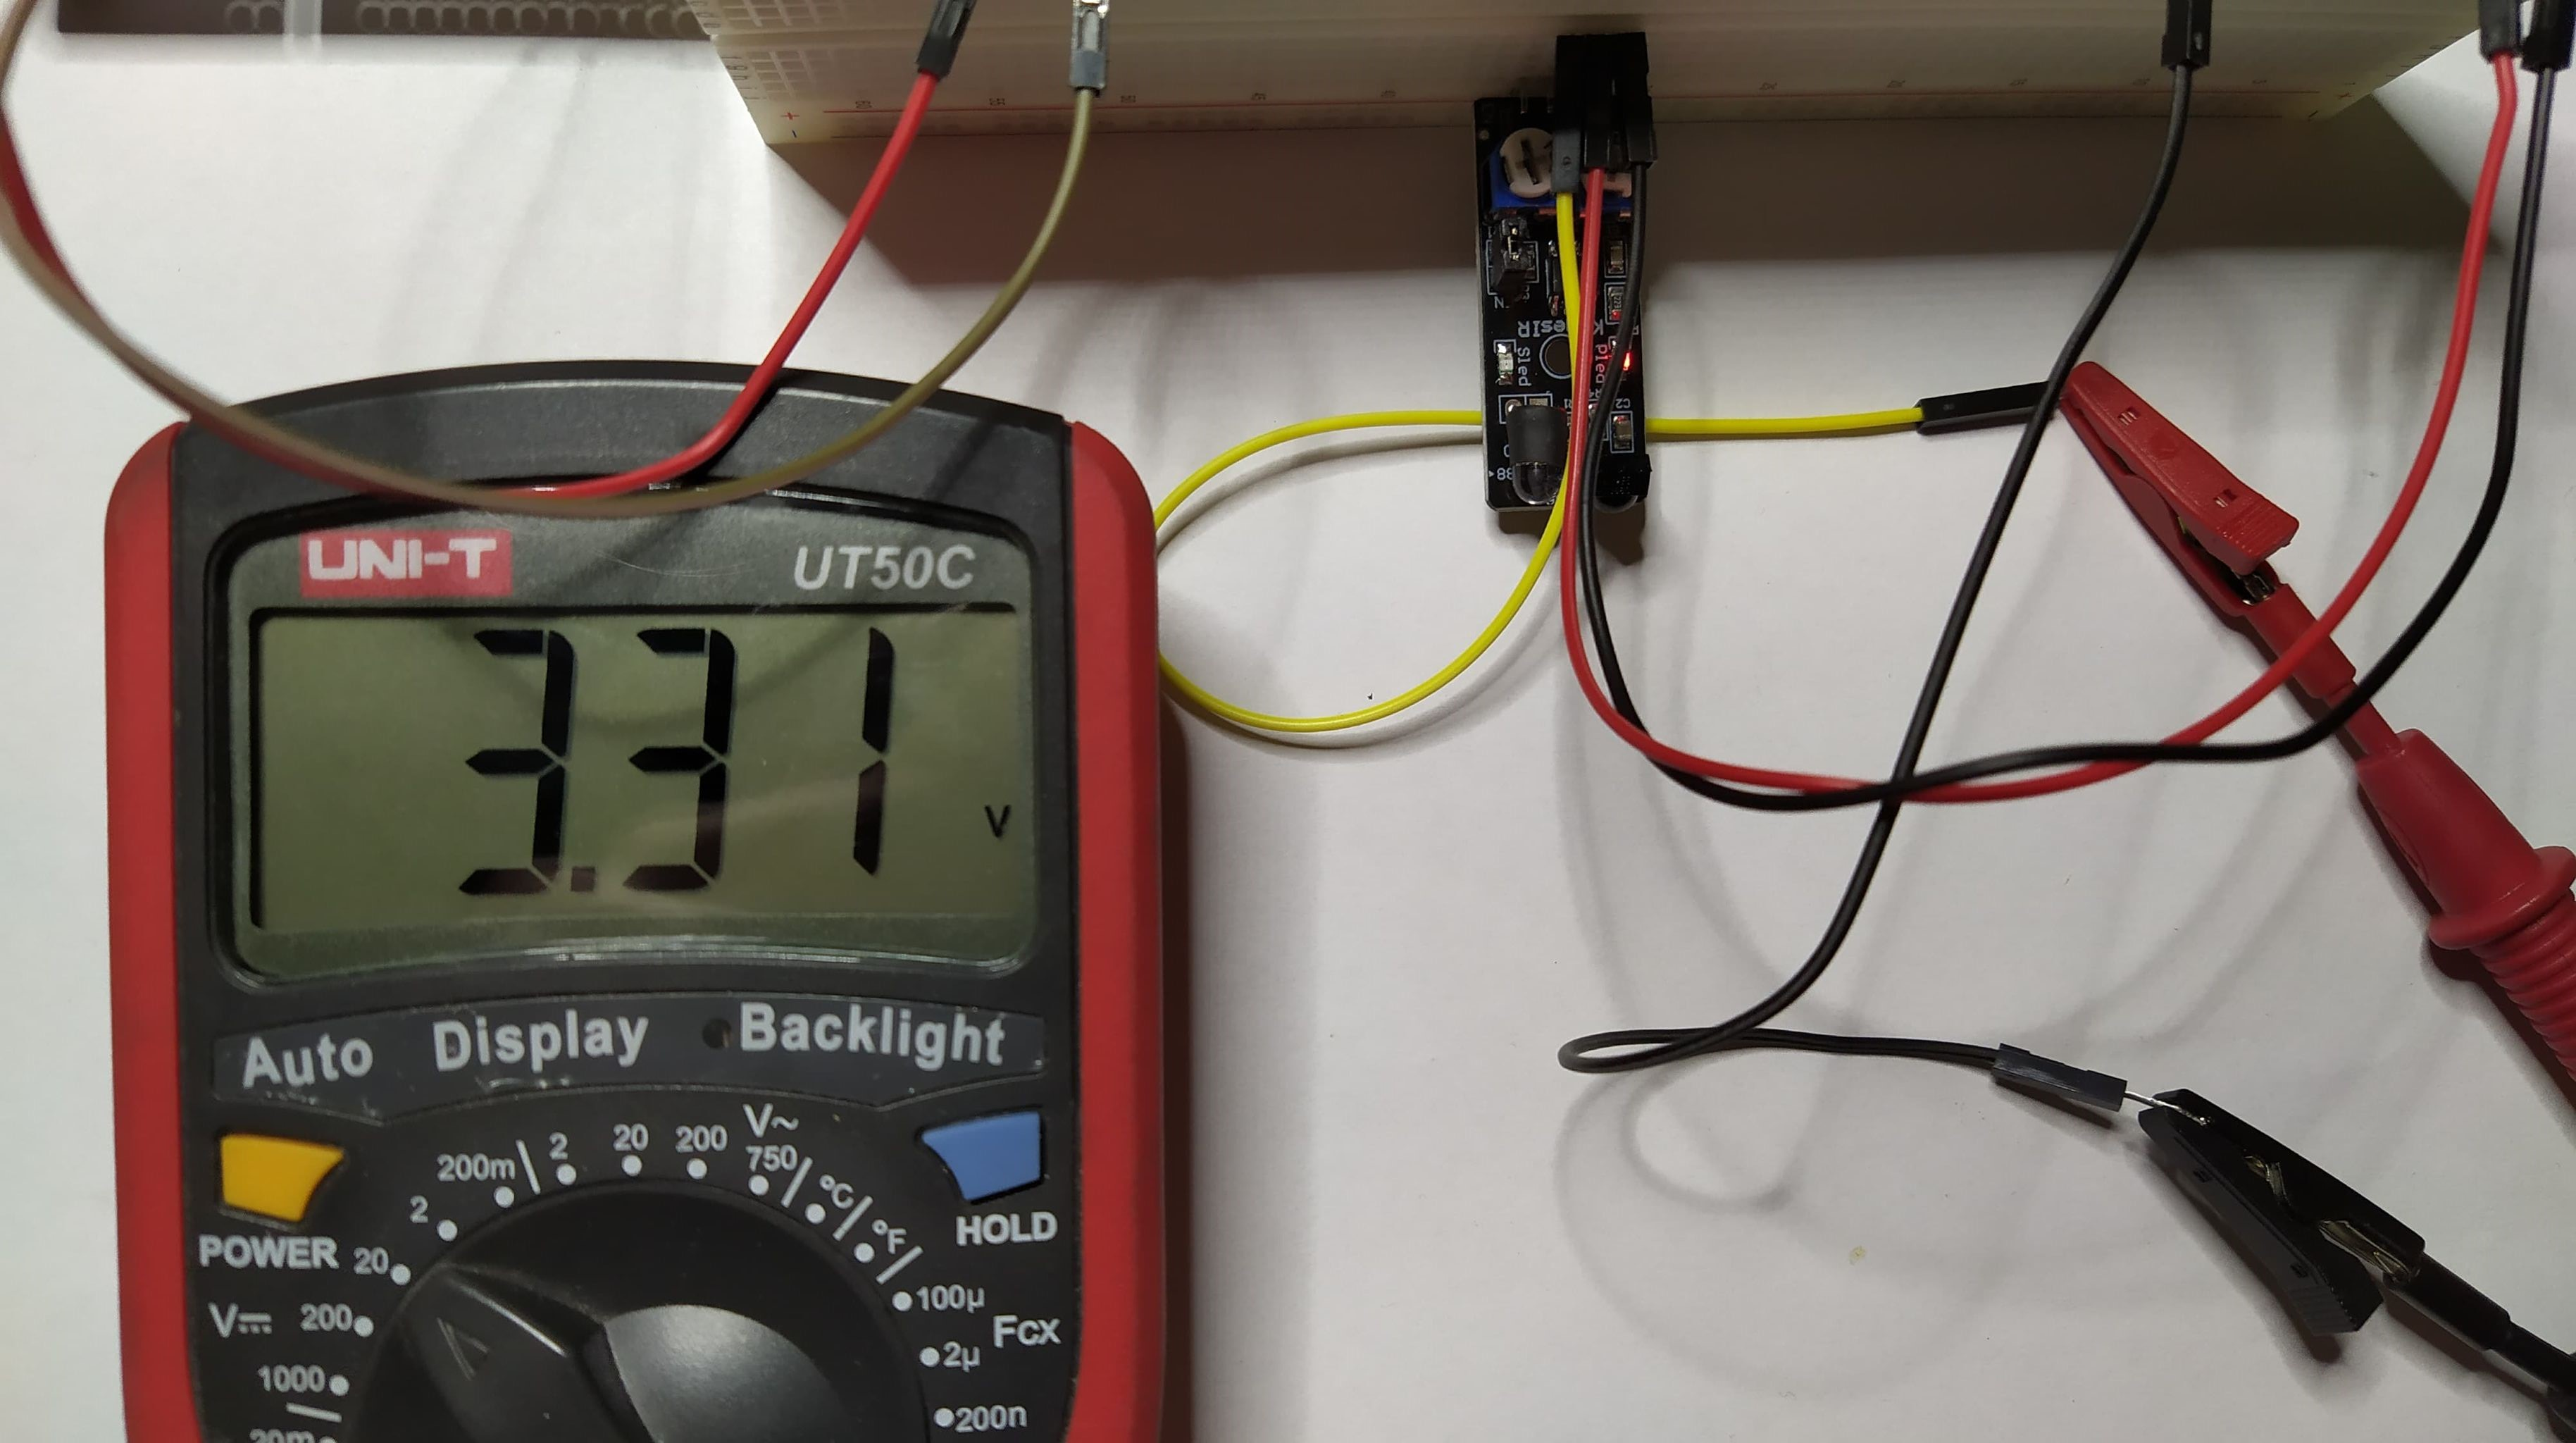
\includegraphics[width=0.7\textwidth]{fig/KY-032/zasada_dzialania/Avoidance_pomiar3.jpg}
    \caption{Pomiar dla braku obiektu przed czujnikiem}
\end{figure}

\newpage

\printbibliography[heading=bibintoc]

\end{document}